\subsection{Comunidade local decisões globais }

\textbf{Cena 5. Junho de 2017. Rio de Janeiro, RJ.}

A disciplina ``Estudos CTS (Ciências-Tecnologias-Sociedades): aproximações brasileiras e latino-americanas'' é ministrada no Programa de Engenharia de Sistemas e Computação da COPPE/UFRJ no 2º período de 2017. A turma é convidada a ler o capítulo 7 do livro ``\textit{Yes, nós temos Pasteur. Manguinhos, Oswaldo Cruz e a história da ciência no Brasil}'' \citep{cukierman_pasteur_2007}, intitulado ``\textit{Prata Preta}''.

``\textit{Chamava-se Horácio José da Silva, mas, que importava?}'' \citep[p. 220]{cukierman_pasteur_2007}. A frase que abre o capítulo citado se refere ao Prata Preta, um personagem da Revolta da Vacina ocorrida no Rio de Janeiro, em 1904, que, como tantos outros tipos, não é encontrado nas narrativas universalizantes da história da ciência brasileira. A leitura, que narra momentos decisivos para a construção sociotécnica das ciências brasileiras pelo ângulo de um personagem que não pensaríamos \textit{a priori} como protagonista, provoca algumas reflexões: a quantos outros/as anônimos/as da história da ciência e tecnologia brasileiras a frase de abertura poderia se referir? Como se faz educação em ciências contextualizada em um país com tantos/as atores/atrizes sem voz? Em espaços populares, fora das salas de aulas dos programas de pós-graduação, quais histórias são contadas e quais versões são aprendidas?

Após a leitura, com todas essas perguntas na cabeça, recebo uma provocação de meu colega de pós-graduação, o doutorando Fernando Severo: ``\textit{vamos melhorar o verbete sobre o Prata Preta na Wikipédia?}''. Imediatamente aceito o convite e vamos analisar o material já existente na enciclopédia. Percebemos então que o verbete biográfico de Prata Preta possuía apenas 1754 bytes\footnote{Unidade de medida utilizada pela comunidade Wikimedia para medir o tamanho de revisões e verbetes.}, sendo a metade deles sobre um bloco de carnaval que leva seu nome.

\begin{figure}[H]
    \centering
    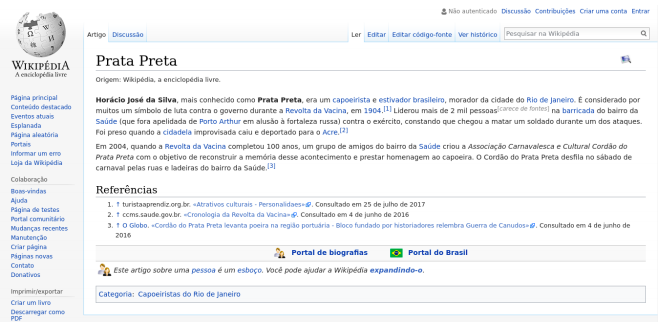
\includegraphics[width=1\textwidth]{Images/pratapreta.png}
    \caption{Versão do verbete Prata Preta encontrado no dia da cena.}
    \label{fig:verbete_pratapreta}
\end{figure}

Aceito o desafio de melhorar o verbete e, enquanto penso sobre os desafios de escrever uma biografia de um subalterno sem voz, com poucas fontes secundárias fiáveis versando sobre sua história, faço uma singela edição com pequenos ajustes ao texto que já estava lá. Para minha grande surpresa, a edição não é salva pela Wikipédia, que me informa: ``\textit{Seu IP está bloqueado}''.

Rapidamente descubro que na verdade não só eu, como milhares de usuários/as da Virtua, maior provedora de internet do Rio de Janeiro, já estavam bloqueados/as por três meses, como resposta a um suposto vandalismo excessivo feito em vários idiomas pelo mesmo range de IP. Essa drástica medida é tomada quando se entende que uma ação orquestrada de vandalismo estará se aproveitando de um provedor de acesso, VPN\footnote{Do inglês Virtual Private Network. São conexões entre máquinas na internet que direcionando o tráfego de uma sempre para a outra.} ou Proxy para mudar de IP constantemente e furar o bloqueio individual a um determinado IP individualizado. E pior, diferente da estratégia de bloqueio simples de IP, onde basta o/a editor/a criar uma conta de usuário/a para (agora rastreado) poder voltar a editar, o bloqueio de faixa de IP incluía também usuários/as registrados/as. Com isso, mesmo meu usuário, com milhares de edições e ficha corrida limpa na enciclopédia, estava proibido de editar.

Fomos então estudar o histórico de edições feitas em nossa faixa de IP e nos surpreendemos com o resultado! Como pode um usuário holandês, que aplicou o bloqueio em todos os sites do Movimento Wikimedia, ter colocado no mesmo balaio de gato Fernando Severo, eu, o IP 179.210.26.120, que estava escrevendo sobre uma escola de samba teresopolitana em português, e o IP 179.210.99.239, que editava sobre a série televisiva ``Meu Pequeno Pônei'' em galego? Não terá seu olhar saxão sido capaz de perceber a distância entre interesses tão distintos e ações de edição? Terá ele conseguido ver apenas uma horda anárquica subdesenvolvida que não tem modos nem educação para escrever uma enciclopédia!?

Saímos então da periferia que é a Wikipédia lusófona e fomos buscar os centros globais de tomada de decisão da enciclopédia. Estudamos as políticas de acesso e de bloqueio globais da comunidade Wikimedia e fomos parar em uma sala de chat em inglês no IRC.\footnote{Do inglês \textit{Internet Relay Chat}, ferramenta para criação de salas de bate papo virtuais.} Lá conversamos com os/as ``gringos/as'', relatando detalhadamente ``o causo'', procurando esclarecê-los a respeito da estrutura do mercado de internet no Rio de Janeiro, com milhões de usuários/as e poucos provedores de acesso; das diversas edições feitas em diferentes wikipédias por editores em nosso range de IP; da forma dinâmica como funciona a distribuição de IP nos provedores de internet; do longo histórico de bom comportamento de meu usuário. Vários/as aliados/as foram convocados/as ao esforço de demonstrar que nosso grupo nada homogêneo, unido involuntariamente por uma faixa de endereços de IP, tem seu valor para a comunidade, e pode ser produtor de conhecimento. Recebi uma desanimadora resposta burocrática de um anglófono, que simplesmente mandou enviar e-mail para um determinado endereço e esperar por um resposta sem prazo.

Mas, eis que de onde parecia que não surgiria mais alento, emerge a empatia de um \textit{steward}\footnote{No Movimento Wikimedia são usuários com permissões para administrar todas as wikis de todos os projetos.} falando português. Ele se solidariza com nosso pleito e nos autoriza a participar novamente do jogo global de construção de conhecimentos na wiki universal, relaxando parcialmente o bloqueio. Agora, após nossa expedição exploratória da implementação da política de bloqueios globais do Movimento durar toda a madrugada, poderíamos novamente editar, desde que estivéssemos devidamente registrados no site com um usuário próprio. Usuários/as anônimos/as continuariam impedidos/as de editar. Afinal, nosso pleito ``tinha seu valor sim, mas também não era para tanto, né?''. Com a confirmação de que havíamos conseguido superar a pane, compondo um novo arranjo suficiente para estabilizar o funcionamento da Wikipédia para nossos usuários, fomos dormir às 5 horas da manhã, sem realizar nenhuma edição no verbete de Prata Preta.